\section{ХОД РАБОТЫ}
\subsection{Теоретические сведения}

Учетная запись пользователя, представляющая собой уникальный личный код,
является основой защиты Windows NT. Создание учетных записей пользователей
и групп занимает важное место в обеспечении безопасности Windows 2000.

Как правило, в процессе установки Microsoft Windows автоматически
создаются две встроенные учетные записи пользователей --- Администратор (Administrator)
и Гость (Guest).

Учетная запись Администратор  используется при установке
и настройке рабочей станции или сервера. Она не может быть уничтожена,
блокирована или удалена из группы Администраторы (Administrators),
ее можно только переименовать.

Учетная запись Гость применяется для регистрации на компьютере без использования
специально созданной учетной записи и предназначена для доступа к ресурсам
компьютера случайных пользователей. Учетная запись Гость не требует ввода пароля
и по умолчанию блокирована. Ей можно предоставить права доступа к ресурсам системы
точно так же, как и при создании любой другой учетной записи с помощью
оснастки Локальные пользователи и группы.

Группа  представляет сбой набор учетных записей пользователей с похожими служебным
обязанностями или потребностями в ресурсах. В процессе установки Microsoft Windows
автоматически создаются шесть следующих встроенных групп:
\begin{enumerate}

\item Администраторы (Administrators) --- ее члены обладают полным доступом
ко всем ресурсам системы. Это единственная встроенная группа,
автоматически предоставляющая своим членам весь набор встроенных прав.

\item Операторы архива (Backup Operators) --- члены этой группы могут
архивировать и восстанавливать файлы в системе независимо от того,
какими правами эти файлы защищены. Кроме того, операторы архива могут
входить в систему и завершать ее работу,
но они не имеют права изменять настройки безопасности.

\item Гости (Guests) --- эта группа позволяет выполнить регистрацию
пользователя с помощью учетной записи Гость и получить ограниченные
права на доступ к ресурсам системы.
Члены этой группы могут завершать работу системы.

\item Опытные пользователи (Power Users) --- члены этой группы могут
создавать учетные записи пользователей и модифицировать настройки безопасности
для созданных ими учетных записей. Кроме того, они могут создавать
локальные группы и модифицировать состав членов созданных ими групп.
То же самое они могут делать с группами Пользователи, Гости и Опытные пользователи.
Члены группы Опытные пользователи не могут модифицировать членство в группах
Администраторы и Операторы архива. Они не могут архивировать или восстанавливать
каталоги, загружать и выгружать драйверы устройств и
модифицировать настройки безопасности и журнал событий.

\item Репликатор (Replicator) --- членом группы Репликатор должна
быть только учетная запись, с помощью которой можно зарегистрироваться
в службе репликации контроллера домена. Ее членами не следует
делать рабочие учетные записи.

\item Пользователи (Users) --- члены этой группы могут выполнять большинство
пользовательских функций, например, запускать приложения, пользоваться локальным
или сетевым принтером, завершать работу системы или блокировать рабочую станцию.
Они также могут создавать локальные группы и регулировать состав их членов.
Они не могут получить доступ к общему каталогу или создать локальный принтер.
\end{enumerate}


\subsection{Создание локальной учётной записи}

Создание учетных записей пользователей и групп в MS Windows осуществляется
с использованием оснастки Локальные пользователи и группы (Local Users and Groups),
которая является инструментом ММС и позволяет выполнять управление локальными
учетными записями пользователей и групп.

Для создания учетной записи пользователя в оснастке Локальные пользователи и группы
установили указатель мыши на папку Пользователи и нажали правую кнопку.
В появившемся контекстном меню выбрали команду Новый пользователь (New User).
Появилось окно диалога Новый пользователь (New User).
Введем имя создаваемого пользователя, полное имя создаваемого пользователя,
описание создаваемого пользователя или его учетной записи.
В поле Пароль введем пароль пользователя подтвердим его правильность
вторичным вводом (рисунок 1). Результат проделанной операции представлен на
рисунке~\ref{pic:user_creation}.
\begin{figure} [h!]
  \centering
  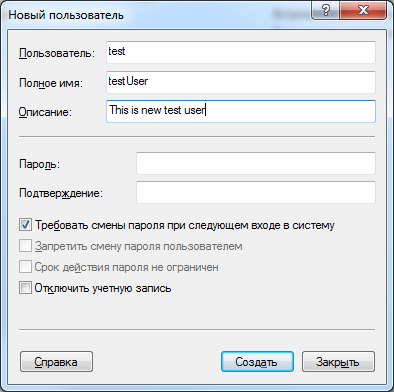
\includegraphics[width=0.9\linewidth]{pic/user_creation}
  \caption{Создание новой учётной записи}
  \label{pic:user_creation}
\end{figure}

\newpage

Для создания локальной группы в окне оснастки Локальные пользователи и группы
установили указатель мыши на папке Группы и нажали правую кнопку.
В появившемся контекстном меню выбрали команду Новая группа (New Group).
Процесс создания новой группы представлен на рисунке~\ref{group_creation}.
\begin{figure} [h!]
  \centering
  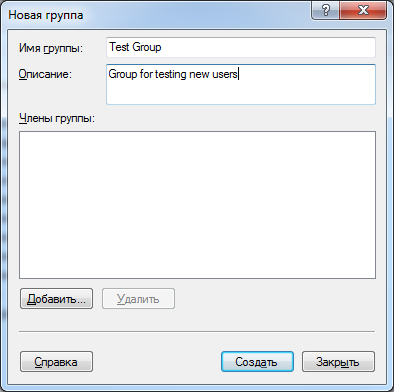
\includegraphics[width=0.7\linewidth]{pic/group_creation}
  \caption{Создание локальной группы пользователей}
  \label{pic:group_creation}
\end{figure}


\subsection{Создание локальных профилей пользователей}

Локальный профиль пользователя хранится на компьютере в папке профиля пользователя,
имя которой совпадает с именем данного пользователя и находится в папке Documents and Settings.
В папке профиля пользователя содержатся подпапки, приведенные в таблице~\ref{tbl:local_profile},
а также файл NTuser.dat и файл журнала транзакций с именем NTuser.dat.LOG,
который позволяет Windows восстанавливать данного профиль пользователя
в случае сбоя при модификации содержимого файла NTuser.dat.

\begin{table} [h!]
  \caption{
    Содержимое папки локального профиля пользователя
  }\label{tbl:local_profile}
  {\small
    \begin{tabular}{| m{4cm} | m{11.6cm} |}
      \hline
      \parbox{4cm}{
          \smallskip
          \centering Наименование подпапки
          \smallskip
        }
      & \parbox{11.6cm}{
          \smallskip
          \centering Содержимое подпапки
          \smallskip
        }
      \\
      \hline

      Application Data &
      Данные, относящиеся к конкретному приложению. Разработчики приложений сами
      принимают решение, какие данные должны быть сохранены в папке профиля пользователя. \\
      \hline

      Cookies &
      Служебные файлы, получаемые с
      просматриваемых веб-серверов. \\
      \hline

      Local Settings &
      Данные о локальных настройках, влияющих на работу программного обеспечения компьютера. \\
      \hline

      NetHood &
      Ярлыки объектов сетевого окружения. \\
      \hline

      PrintHood &
      Ярлыки объектов папки принтера. \\
      \hline

      Recent &
      Ярлыки недавно используемых объектов. \\
      \hline

      SendTo &
      Ярлыки объектов, куда могут посылаться документы. \\
      \hline

      Главное меню (Start Menu) &
      Ярлыки установленных программ. \\
      \hline

      Избранное (Favorites) &
      Ярлыки часто используемых программ и папок. \\
      \hline

      Мои документы \newline (My Documents) &
      Данные о документах и графических файлах, используемых пользователем. \\
      \hline

      Рабочий стол \newline (Desktop) &
      Объекты рабочего стола, включая файлы и ярлыки. \\
      \hline

      Шаблоны (Template) &
      Ярлыки шаблонов. \\
      \hline

    \end{tabular}
  }
\end{table}

При первой регистрации для пользователя, у которого не существует сконфигурированного
перемещаемого профиля (этот профиль находится на сервере),
создается индивидуальный профиль. Содержимое папки Default User копируется в папку
нового профиля пользователя. Данные профиля, вместе с содержимым папки All Users
используется при конфигурации рабочей среды пользователя. По завершении работы
на компьютере все изменения настроек рабочей среды сделанные пользователем
записываются в его профиль, при этом содержимое папки Default User остается неизменным.

Если пользователь имеет отдельную учетную запись на локальном компьютере и в домене,
то для каждой из них создается свой профиль пользователя, так как регистрация
на компьютере происходит с помощью различных учетных записей.


\subsection{Создание сценариев входа}

Обычно сценарий входа является пакетным файлом, который автоматически
выполняется при каждом входе пользователя в систему. Сценарии входа используются
для настройки рабочей среды пользователя при входе и позволяют администратору
задавать основные параметры рабочей среды пользователя, не участвуя
непосредственно во всех настройках. Сценарий входа может быть присвоен одной
или нескольким учетным записям пользователей.

Во время входа пользователя в систему проверяющий сервер обычно ищет сценарий
входа в систему (если таковой был связан с учетной записью пользователя) по
следующему пути: Системный <<Корневой Каталог \ System32 \ Repl \ Import \ Scripts>>.
Для назначения сценария входа учетной записи пользователя, в оснастке
Локальные пользователи и группы установили указатель мыши на папку Пользователи
и нажали левую кнопку. Выбрали требуемого пользователя и на вкладке
Профиль окна свойств учетной записи этого пользователя в поле
Сценарий входа (Logon Script) представлен на рисунке~\ref{pic:scenario_creation}.
\begin{figure} [h!]
  \centering
  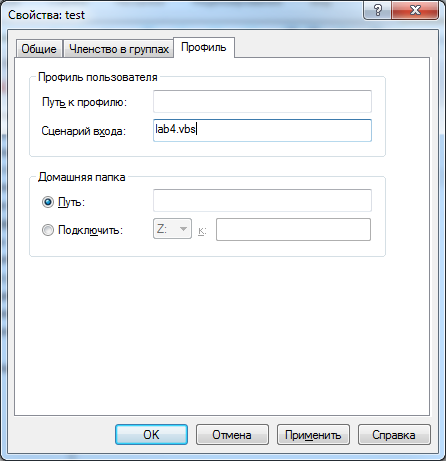
\includegraphics[width=0.6\linewidth]{pic/scenario_creation}
  \caption{Создание сценария выполнения автозагрузки приложений}
  \label{pic:scenario_creation}
\end{figure}


При входе в систему должен выполняться сценарий входа ---
пакетный файл «lab4.bat» с содержимым, приведенным на рисунке~\ref{lst:lab_4_bat}.
\begin{lstlisting}[caption={Содержимое файла <<lab4.bat>>},
label=lst:lab_4_bat]
 @echo off
 wscript %0\..\lab4.vbs
\end{lstlisting}

Данный скрипт запускает на выполнение код, написанный на VBScript. Пример кода
на VBScript приведен на рисунке~\ref{lst:vbscript}.
\begin{lstlisting}[caption={Содержимое файла <<lab4.bat>>},
label=lst:lab_4_bat]
 Option Explicit
 Dim WshShell, theCalculator, PathTarg
 Set WshShell = WScript.CreateObject("WScript.Shell")
 Set theCalculator = WshShell.Exec("calc")
 WScript.Sleep 500
 WshShell.AppActivate theCalculator.ProcessID
 PathTarg=WshShell.ExpandEnvironmentStrings("%homepath%")
 MsgBox(PathTarg)
\end{lstlisting}

Приведенный скрипт запускает калькулятор и выводит на экран настройки среды
пользователя. Теперь следует поместить эти два файла в каталог <<c://windows/system32/Repl/Import/Scripts>>.
Таким образом, при последующем входе пользователя <<Администратор>> в сеть
будут запускаться два приложения.
